% !TEX encoding = UTF-8 Unicode
% \documentclass{article}
% \usepackage{../../superstyle}
% \usepackage{listings}
% \usepackage{amsmath}
% \begin{document}
% remove all before

%oppgavetekst
Rerun the calculation in Step 1 for $n = 10\cdot2^k$, where k = 1,...,11. Make a table of the errors at x = L for each n. For which n is the error smallest? Why does the error begin to increase with n after a certain point? You may want to make an accompanying table of the
condition number of A as a function of n to help answer the last question. To carry out this step for large k, you may need to ask Matlab to store the matrix A as a sparse matrix to avoid running out of memory. To do this, just initialize A with the command A=sparse(n,n), and proceed as before. We will discuss sparse matrices in more detail in the next section.

\vspace{5mm}
Løsning

\begin{lstlisting}[caption={oppgave3.m}]
feiltab = zeros(11,1); 
kondtab = zeros(11,1); 
for(eksp=1:11)
    n=10*(2.^eksp);
    tall1 = lagmatrise(n)\konstantkrefter(n);
    tall2 = korrektutregning(n);
    tall3 = tall1(n)-tall2(n); 
    feiltab(eksp) = tall3; 
    kondtab(eksp)=condest(lagmatrise(n));
end;
disp('Feilene er som følger:'); 
disp(feiltab); 
disp('Kondsisjonstallene er som følger: ') ; 
disp(kondtab); 
\end{lstlisting}

\vspace{3mm}

\begin{figure}[h]
\centering
\begin{minipage}{.5\textwidth}
  \centering
  % \includegraphics[width=0.5\textwidth]{result3}
  \includegraphics[width=0.8\textwidth]{sections/Exercise3/result3}
    \caption{Errors}
    \label{fig:errors3}
\end{minipage}%
\begin{minipage}{.5\textwidth}
  \centering
  % \includegraphics[width=0.7\textwidth]{cond3}
  \includegraphics[width=0.8\textwidth]{sections/Exercise3/cond3}
    \caption{Condition Numbers}
    \label{fig:cond3}
\end{minipage}
\end{figure}
 
Feilene vises i figur \ref{fig:errors3}, og man kan se at feilen øker når n øker, dette kan man se har en sterk sammenheng med kondisjonstallene som vist i figur \ref{fig:cond3}. Den minste feilen er når k = 1, altså når $n = 10\cdot2^1 = 20$.


% remove after
% \end{document}